\chapter{Extrakcia príznakov a ich klasifikácia}
\label{kap:features}
V kapitole ukážeme riešenie problému klasifikácie osôb na základne extrahovaných príznakov zo snímok celého tela týchto osôb.
Naše riešenie preberá niektoré myšlienky z práce Person Re-identification by Local Maximal OccurrenceRepresentation and Metric Learning \cite{featuresinspiration}, detaily riešenia sa však odlišujú.
Ďalej porovnáme dve metódy klasifikácie: pomocou najbližších susedov a pomocou support vector machines.
\section{Dataset}
Využili sme dataset DukeMTMC-reID \cite{ristani2016MTMC} \cite{zheng2017unlabeled}. 
Jedná sa o upravenú verziu datasetu DukeMTMC.
Pôvodný dataset obsahuje videozáznamy z ôsmich rôznych kamier.
V upravenej verzii sú zábery jednotlivých osôb vyrezané z každej stodvadsiatej snímky pôvodného videozáznamu.
Takto je získaných 1 404 identít, ktoré sa vyskytujú aspoň na dvoch kamerách a 408 identít vyskytujúcich sa práve na jednej kamere.
Náhodne vybraná polovica osôb, ktoré sa vyskytujú na viacerých záberoch, je zvolená ako trénovacia množina, zvyšné zábery patria do testovacej množiny.

\begin{figure}[H]
\centerline{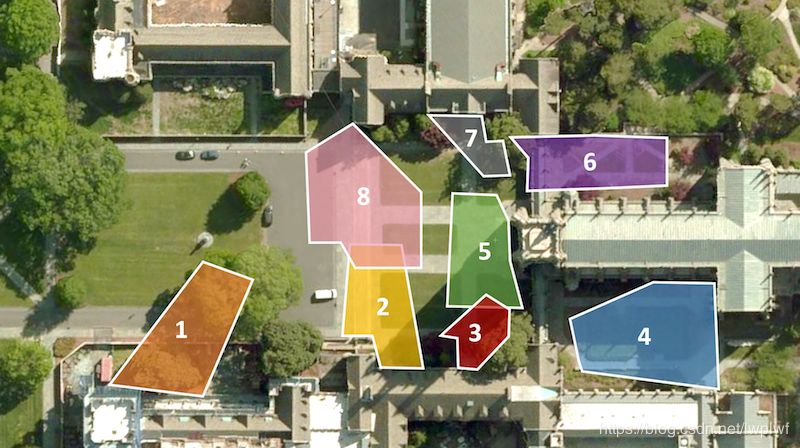
\includegraphics[width=0.9\textwidth]{images/duke_topology}}
\caption[Topológia kamier]{Oblasti, ktoré zachytávajú jednotlivé kamery v datasete DukeMTMC}
\label{obr:duke_topology}
\end{figure}

\begin{figure}[H]
\centerline{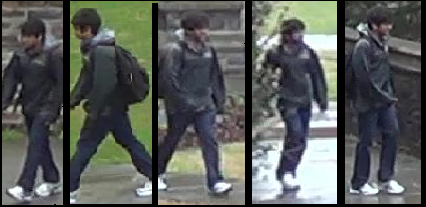
\includegraphics[width=0.9\textwidth]{images/duke_same}}
\caption[Ukážka datasetu]{Zábery jednej osoby z rôznych kamier v datasete DukeMTMC-reID}
\label{obr:duke_same}
\end{figure}

\def\lc{\left\lfloor}
\def\rc{\right\rfloor}

\section{Extrakcia príznakov}
Extrakcia príznakov je metóda redukcie dimenzie elimináciu nepodstatných detailov.
Cieľom je získať množinu príznakov, ktorá pôvodný vstup dobre reprezentuje s menším počtom dát.

\subsection{Lokálny binárny vzor}
Príznaky získané pomocou lokálneho binárneho vzoru sa veľmi často využívajú pri rôznych problémoch klasifikácie.
Jedná sa o dobre overenú metódu, ktorá má navyše nízku výpočtovú náročnosť \cite{lbp}.
Lokálny binárny vzor porovnáva hodnoty každého pixelu s jeho susednými pixelmi.
Má dva parametre.
\begin{description}
\item[Počet sudedov $P$] Určuje, s koľkými susednými pixelmi obrázku budeme porovnávať každý pixel.
\item[Polomer $R$] Polomer kružnice, na ktorej ležia susedia, pričom určíme, že pixel má tvar štvorca s dĺžkou strany 1.
\end{description}
Pokiaľ chceme susedov, s ktorými ma pixel spoločnú hranu, nastavíme P=4 a R=1.
Ak by sme chceli susedov so spoločným vrcholom pomyselného štvorca, nastavíme P=8 a R=1.

Lokálny binárny patern spočíta pre každý pixel $I$ s hodnotou $V_I$ a so susedmi $I_0$,\,...,\,$I_{P-1}$ čiernobieleho obrázku hodnotu $LBP(I)$,
$$LBP(I) = \sum_{n=0}^{P-1} s(V_I - V_{I_n})*2^n $$


\[
  s(k) =
  \begin{cases}
    0 & \text{ak $k < 0$} \\
    1 & \text{ak $k \geq 0$}
  \end{cases}
\]

Môžeme so všimnúť, že takto získané číslo bude mať hodnotu z intervalu prirodzených čísel $<0, 2^P)$.

  
\subsection{Lokálny ternárny vzor}
Funguje podobne ako lokálny binárny vzor \cite{ltp}.
Ak už názov napovedá, pri porovnávani namiesto dvoch hodnôt vyhodnocuje na tri hodnoty.
Má navyše ešte jeden parameter.
\begin{description}
\item[Threshold $T$] Podľa thresholdu sa určí výsledná hodnota pri porovnávaní
\end{description}
$$LTP(I) = \sum_{n=0}^{P-1} s(V_I, V_{I_n})*3^n $$
\[
  s(c, p) =
  \begin{cases}
    2 & \text{ak $c + T < p$} \\
	1 & \text{ak $c + T > p$} \\
	0 & \text{inak} 
  \end{cases}
\]
Môžeme so všimnúť, výsledok bude z intervalu prirodzených čísel $<0, 3^P)$.
Väčšie rozpätie intervalu môžu v praxi znamenať lepšie výsledky \cite{ltp}.

Škálovo invariantný lokálny ternárny vzor je rozšírením lokálneho ternárneho vzoru.
Jeho výhodou je, že sa dokáže vysporiadať s jemnými zmenami osvletlenia na snímkach.
Tieto zmeny môžu byť na celej snímke alebo aj len na jej častiach \cite{siltp}. 
$$SILTP(I) = \sum_{n=0}^{P-1} s(V_I, V_{I_n})*3^n $$
\[
  s(c, p) =
  \begin{cases}
    2 & \text{ak $(1 + T)*c < p$} \\
	1 & \text{ak $(1 - T)*c > p$} \\
	0 & \text{inak} 
  \end{cases}
\]

\subsection{Využitie viacrozmerného HSV histogramu pri extrakcii príznakov}
Pri hľadaní osoby, ktorú sme stratili z dohľadu, môže byť dobrým príznakom, podľa ktorého sa nám podarí tú istú osobu opätovne nájsť, farba.
Veľkú plochu človeka pokrýva oblečenie, ktoré ma vo veľa prípadoch rovnakú farbu z každej strany.
To znamená, ak budeme vyhľadávať osobu podľa farby, nezáleží nám, z akého uhlu osobu zachytíme.

Rozpoznávať len podľa farby však rozhodne nie je dobré riešenie.
Človek môže mimo záberu kamery oblečenie zmeniť, hlavne ak sú zábery zachytené s väčším časovým rozdielom.
Takisto problém môžu spôsobiť dve rôzne osoby s rovnakou farbou oblečenia.

Snímky najskôr prekonvertujeme do farebného modelu HSV.
Model HSV sa v oblasti počítačového videnia využíva z dôvodu, že v praxi dosahuje lepšie výsledky ako model RGB \cite{RGBHSV}.
Na zachytenie farby na snímkach využijeme viacrozmerný histogram.
Histogram má rozmer 8x8x8.
Nech pixel obrázku má HSV hodnoty $(h,s,v)$, ktoré patria do intervalu $<0, 255>$
Potom výskyt týchto hôdnot daného pixelu bude v histograme zaznamenaný na indexe $\lc \frac{8h}{256} \rc$ prvej dimenzie, $\lc \frac{8s}{256} \rc$ druhej dimenzie a $\lc \frac{8v}{256} \rc$ tretej dimenzie.


Obrázok, z ktorého extrahuje príznaky rozdelíme na regióny veľkosti 10x10 pixelov, pričom sa tieto regióny prekrývajú na piatich pixeloch.
V každom regióne vytvoríme viacrozmerný HSV histogram.
Pre redukciu dimenzie výstupného vektora príznakov spojíme histogramy regiónov jedného riadku tak, že výsledný histogram bude mať jednotlivé výskyty hodnôt maximalizované (výskyt hodnoty výsledného histogramu daného riadku regiónov je rovný maximálnemu výskytu tej istej hodnoty v danom riadku).
Dôležité však je, že ak sa osoba nachádzádzala na rôznych snímkach na iných častiach týchto snímok (napríklad na jednej snímke mohla byť viac vpravo ako na druhej snímke), výsledný histogram bude pre obe snímky rovnaký. 
Presnejšie povedané, výskyty hodnôt, ktoré sú získane z časti obrázku, na ktorom sa osoba nachádza, budú v oboch histogramoch približne rovnaké.

\subsection{Využitie skálovo invariantného lokálneho ternárneho vzor pri extrakcii príznakov}
Rovnako, ako pri využití viacrozmerného HSV histogramu, tentokrát čiernobiely obrázok rozdelíme na regióny.
Na každom regióne aplikujeme škálovo invariantný lokálny ternárny vzor najskôr s parametrami $P=4$, $R=3$, $T=0,3$ a následne aj $P=4$, $R=5$, $T=0,3$. 
Tieto hodnoty sa ukázali pri testovaní ako najlepšie a sú rovnaké, aké boli použité už v spomenutej práci alebo aj iných podobných prácach \cite{featuresinspiration}.
Následne zostrojíme (jednorozmerný) histogram zo získaných hodnôt jednotlivých pixelov, ktorý po riadkoch maximalizujeme rovnako, ako v predchádzajúcej podkapitole.
Keďže hodnoty sú z intervalu $<0, 80>$, v histograme zaznamenáme výskyt každej hodnoty samostatne.
Hodnota $i$ bude zaznamenaná na indexe $i$.


\subsection{Algoritmus retinex}
Aj keď škálovo invariantný lokálny ternárny vzor a farebný model HSV čiastočne riešia zmeny osvetlenia medzi zábermi rovnakej, ale aj rôznych kamier, rozhodli sme sa na predspracovanie snímok použiť aj algoritmus retinex.
Jeho úlohou je tieto zmeny odstrániť.
Algoritmus je inšpirovaný biologickými mechanizmamy očí a ich schopnosti adaptovať sa týmto zmenám \cite{retinex}.

\subsection{Analýza hlavných komponentov}
Ak majú snímky, podľa ktorých chceme klasifikovať rozmery 65x155 pixelov, extrakciou príznakov ako sme popísali dostaneme vektor príznakov veľkosti až 20 220 ($(8^3 + 3^4 + 3^4)*(\frac{155-5}{5})$).
Dimenziu tehto vektora môžeme redukovať pomocou analýzy hlavných komponentov (PCA).

Snahou PCA je znížiť dimenziu množiny vektorov s čo najmenšou stratou informácie.
PCA vykoná transfomáciu prvkov vektora, ktoré sú pravdepodobne korelované, na nižší počeť lineárne nezávyslích prvkov, ktoré sa nazývajú hlavné komponenty \cite{pca}.
Vďaka tomu budeme vedieť vykonávať klasifikáciu oveľa rýchlejšie.

\section{Klasifikácia}
Úlohou klasifikácie je identifikovať, do akej množiny kategórií (tried) patrí nové pozorovanie na základne informácií získaných z trénovacej množiny pozorovaní.
\subsection{Metóda k-najbližších susedov}
Metóda k-najbližších susedov je relatívne jednoduchá, no aj tak v mnohých prípadoch účinná klasifikačná metóda \cite{knn}.
Je založená na výpočte vzdialeností medzi vektormi príznakov trénovacích dát a vektorom príznakov pozorovania, ktoré chceme klasifikovať.
Po vypočítaní všetkych vzdialeností pridelíme danému pozorovaniu triedu, ktorá sa vyskystuje najčastejšie v $k$ najbližších (s najmenšou vypočítanou vzdialenosťou) pozorovaniach z trénovacej množiny dát.

Na výpočet vzdialeností sa väčšinou používa euklidovská vzdialenosť.
Hodnota $k$ sa volí relatívne malá a líši sa v závislosti od počtu rôznych tried, počtu pozorovaní v trénovacej množine a podobne. 
Vhodnú hodnotu je možné nájsť experimentovaním \cite{knn}.

Hlavnou nevýhodou je jeho rýchlosť. 
Pri veľa dátach v trénovacej množite je metóda pomalá, keďže je pri každej klasifikácii počítať vzdialenosť pre každé pozorovanie v tejto množine.

\subsection{Metóda podporných vektorov}
Pomocou metódy podporných vektorov (SVM) vieme klasifikovať do dvoch tried.
Príznaky, podľa ktorých chceme klasifikovať, sú reprezentované ako vrcholy v priestore.
Úlohou SVM je nájsť nadrovinu, ktorá tento priestor rozdelí na dva podpriestory, pričom v každom podpriestore sa nachádzajú len príznaky patriace do jednej triedy.
Vzdialenosť všetkých príznakov by mala byť od rozdelovacej nadroviny čo najväčšia.

V prípade, že takáto nadrovina neexistuje, je možné uplatniť transformáciu, ktorá priestor príznakov prevedie do vyššej dimenzie, v ktorej už existovať bude.
V tomto prípade hovoríme o nelineárnom SVM.

Klasifikácia je oproti metóde nejabližších susedov rýchlejšia.
Pokiaľ chceme klasifikovať nové pozorovanie, stačí zistiť, do ktorého podpriestoru patrí nový vektor príznakov.

Klasifikácia do viacerých tried je možná zostrojením SVM pre každú triedu a následnom binárnom rozhodnutí, či príklad patrí do tejto triedy alebo nie \cite{svm}. 
Pr

\subsection{Výsledky}
Z výsledkov testovania vidieť, že využitie retinexu pri klasifikácii pomáha vo všetkých prípadoch.
Metóda najbližších susedov dosahuje najlepšie výsledky pri 300 PCA komponentoch a hľadaní len jedného najbližšieho suseda.
Metóda podporných vektorov dosahuje výrazne lepšie výsledky ako metóda najbližších susedov.
Najlepšie výsledky dosahuje pri 500 PCA komponentoch.

\begin{figure}[H]
\centerline{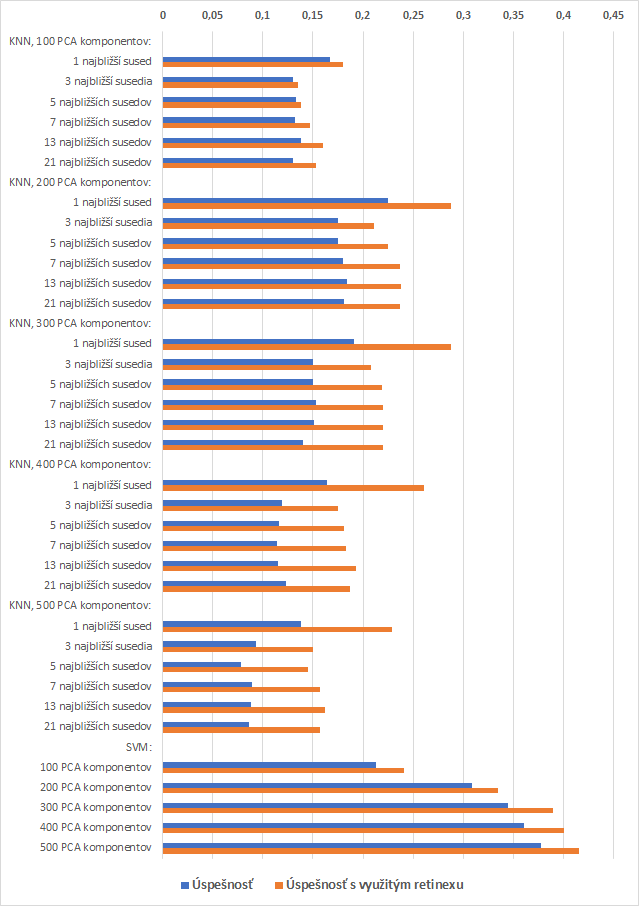
\includegraphics[width=1\textwidth]{images/graph_features_compare}}
\caption[Výsledky porovnania metód]{Graf porovnáva výsledky popísaných riešení s rôznymi parametrami a s využitím a taktiež bez využitia algortimu retinex.}
\label{obr:graph_features_compare.png}
\end{figure}

\section{Porovnanie a diskusia}

V porovnaní s publikovanými riešeniami pre tento dataset dosahujeme slabšie výsledky.
Avšak ani najlepšie riešenia nedosahujú dostatočnú úspešnosť klasifikácie, pokiaľ sa riešenie aplikuje na odlišný dataset \cite{stateofart}.
Pokiaľ chceme vytvoriť systém, ktorý by sa dal využiť na viacerých miestach, bude potrebné iné riešenie.

Ďalšou zjavnou nevýhodou je klasifikácia do dopredu určeného počtu tried, čo prináša problémy bližšie popísané v nasledujúcej kapitole \ref{siam_class}.
Ak by sme chceli riešenie využiť na sledovanie osôb v reálnom čase, riešenie je navyše pomalé.
Extrakcia príznakov a ich následná klasifikácia zaberie na jednej snímke približe sekundu.

\begin{figure}[H]
\centerline{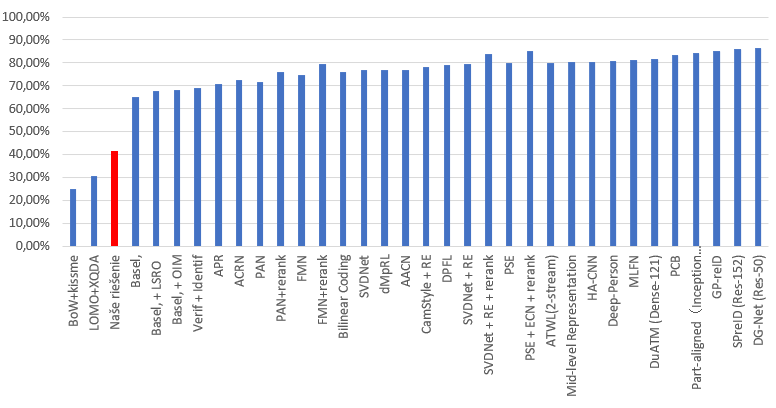
\includegraphics[width=1\textwidth]{images/graph_duke_compare}}
\caption[Výsledky publikovaných riešení v porovnaní s naším riešením]{Graf porovnáva úspešnosť klasifikácie nášho najlepšieho riešenie (zobrazeného červenou farbou) s ostatnými zverejnenými riešeniami \cite{stateofart}.}
\label{obr:graph_duke_compare.png}
\end{figure}


\begin{figure}[H]
\centerline{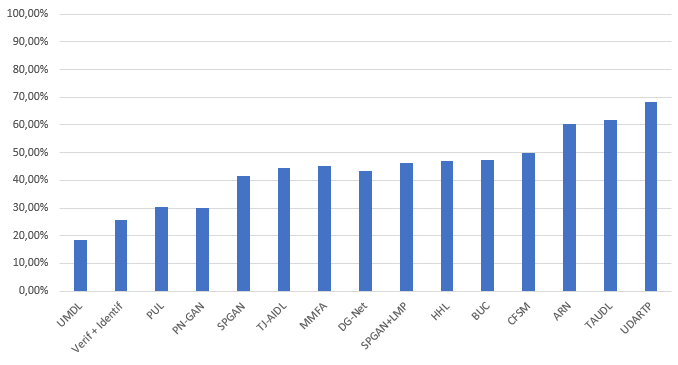
\includegraphics[width=1\textwidth]{images/graph_duke_different}}
\caption[Výsledky publikovaných riešení pri testovaní na odlišnom datasete]{Graf ukazuje úspešnosť klasifikácie riešení natrénovaných na datasete Market-1501 a testovaných na DukeMTMC-reID \cite{stateofart}.}
\label{obr:graph_duke_different.png}
\end{figure}